\documentclass[fleqn, 11pt]{article}\usepackage[]{graphicx}\usepackage[]{color}
% maxwidth is the original width if it is less than linewidth
% otherwise use linewidth (to make sure the graphics do not exceed the margin)
\makeatletter
\def\maxwidth{ %
  \ifdim\Gin@nat@width>\linewidth
    \linewidth
  \else
    \Gin@nat@width
  \fi
}
\makeatother

\definecolor{fgcolor}{rgb}{0.345, 0.345, 0.345}
\newcommand{\hlnum}[1]{\textcolor[rgb]{0.686,0.059,0.569}{#1}}%
\newcommand{\hlstr}[1]{\textcolor[rgb]{0.192,0.494,0.8}{#1}}%
\newcommand{\hlcom}[1]{\textcolor[rgb]{0.678,0.584,0.686}{\textit{#1}}}%
\newcommand{\hlopt}[1]{\textcolor[rgb]{0,0,0}{#1}}%
\newcommand{\hlstd}[1]{\textcolor[rgb]{0.345,0.345,0.345}{#1}}%
\newcommand{\hlkwa}[1]{\textcolor[rgb]{0.161,0.373,0.58}{\textbf{#1}}}%
\newcommand{\hlkwb}[1]{\textcolor[rgb]{0.69,0.353,0.396}{#1}}%
\newcommand{\hlkwc}[1]{\textcolor[rgb]{0.333,0.667,0.333}{#1}}%
\newcommand{\hlkwd}[1]{\textcolor[rgb]{0.737,0.353,0.396}{\textbf{#1}}}%
\let\hlipl\hlkwb

\usepackage{framed}
\makeatletter
\newenvironment{kframe}{%
 \def\at@end@of@kframe{}%
 \ifinner\ifhmode%
  \def\at@end@of@kframe{\end{minipage}}%
  \begin{minipage}{\columnwidth}%
 \fi\fi%
 \def\FrameCommand##1{\hskip\@totalleftmargin \hskip-\fboxsep
 \colorbox{shadecolor}{##1}\hskip-\fboxsep
     % There is no \\@totalrightmargin, so:
     \hskip-\linewidth \hskip-\@totalleftmargin \hskip\columnwidth}%
 \MakeFramed {\advance\hsize-\width
   \@totalleftmargin\z@ \linewidth\hsize
   \@setminipage}}%
 {\par\unskip\endMakeFramed%
 \at@end@of@kframe}
\makeatother

\definecolor{shadecolor}{rgb}{.97, .97, .97}
\definecolor{messagecolor}{rgb}{0, 0, 0}
\definecolor{warningcolor}{rgb}{1, 0, 1}
\definecolor{errorcolor}{rgb}{1, 0, 0}
\newenvironment{knitrout}{}{} % an empty environment to be redefined in TeX

\usepackage{alltt}
\usepackage{amsmath}
\usepackage{amssymb}
\usepackage{geometry}
\usepackage{graphicx}
\usepackage{bm}
\usepackage{url}
\usepackage{enumerate}
\usepackage{fullpage}
\IfFileExists{upquote.sty}{\usepackage{upquote}}{}
\begin{document}
\setlength\parindent{0pt}

\begin{center}
\large
\textbf{Lecture 6: Confidence Intervals}\\
\normalsize
\textbf{STAT 630, Fall 2021}\\
\hrulefill
\end{center}

\begin{itemize}
\item \textbf{Point estimate}: our best guess for the value of a population parameter (e.g., $\bar{x}$ is a point estimate of $\mu$).
\item \textbf{Interval estimate}: a plausible range of values for the population parameter.  Similar to point estimates, interval estimates are random and vary from sample to sample.\\    
\end{itemize}

\textbf{Confidence interval for the population mean $\mu$ when the sample size $n$ is large}:\\

Let $X_1, X_2, \cdots, X_n$ be a random sample of size $n$.  For large $n$, the central limit theorem states that $\bar{X} \sim N(\mu, \sigma / \sqrt{n})$.  Using this we can write the following probability statement:
\begin{align*}
P \left( -1.96 < \frac{\bar{X} - \mu}{\sigma / \sqrt{n}} < 1.96 \right) = 0.95\\
\end{align*}
This follows since the $(1-0.95)/2 = 0.025$ quantile of the standard normal distribution is\\ $\texttt{qnorm(0.025)}=-1.96$, which implies $P(-1.96 < Z < 1.96) = 0.95$ for $Z\sim N(0,1)$.\\  Rearranging terms in the above probability statement gives:
\begin{align*}
P(\bar{X} - 1.96 \sigma / \sqrt{n} < \mu < \bar{X} + 1.96 \sigma / \sqrt{n}) = 0.95
\end{align*}
We call $\bar{X} \pm 1.96 \sigma / \sqrt{n}$ a 95\% confidence interval (CI) for the population mean $\mu$.  Specifically, $(\bar{X} - 1.96 \sigma / \sqrt{n}, \bar{X} + 1.96 \sigma / \sqrt{n})$ is a random interval that contains the population mean $\mu$ with probability 0.95.  The interval is random since it is computed from a sample (each sample gives a different interval).\\ 

\textbf{What does 95\% confidence mean?}
Suppose we repeatedly take random samples of size $n$ from the population, and construct a 95\% confidence interval using each sample. Then approximately 95\% of those intervals (19 out of every 20) should contain the population mean $\mu$.\\
\clearpage

\textbf{Remarks}:
\begin{itemize}
\item The population standard deviation $\sigma$ is usually unknown. When $\sigma$ is unknown we can estimate it with the sample standard deviation $s$.  This introduces another source of random error in the intervals we construct since $s$ also varies from sample to sample. However, $\bar{x} \pm 1.96 s / \sqrt{n}$ is a good approximation of $\bar{x} \pm 1.96 \sigma / \sqrt{n}$ when the sample size is large ($n \geq 30$), and when the population distribution is not too heavily skewed or non-normal. 
\item For a \textbf{given realization} of a confidence interval (i.e., the interval is calculated using values from a single, observed sample) it is incorrect to say that there is a 0.95 probability that the population mean $\mu$ is contained in that interval.  Since $\mu$ is a fixed number, it is either contained or not contained in the interval calculated using a given sample. Instead, we say that we are 95\% confident that $\mu$ is contained in the interval.  
\end{itemize}
\vspace{11pt}

\textbf{Ex1}:  A random sample of 100 US high school students were asked, ``How many days were you physically active for over an hour in the last 7 days?"  The sample mean was $\bar{x} = 3.75$ days with a standard deviation of $s=2.6$ days.\footnote{Data from the Youth Risk Behavior Surveillance System (YRBSS): \url{https://www.cdc.gov/healthyyouth/data/yrbs/data.htm}}  Calculate and interpret a 95\% confidence interval for the population mean number of physically active days per week for high school students in the US.\\  
% \vspace{7.5cm}

{\color{blue}
Given $n=100$, $\bar{x} = 3.75$, $s = 2.6$\\
Sine $n$ is large, a 95\% confidence interval can be calculated as
$$\bar{x} \pm 1.96 \frac{s}{\sqrt{n}} \implies
3.75 \pm 1.96 \cdot \frac{2.6}{\sqrt{100}} \implies
(3.24, 4.26)$$
We are 95\% confident that the population mean, $\mu$, is between 3.24 and 4.26 days.\\
}
\vspace{2cm}

\textbf{Ex2}:  Critique the following statement:  There is a 0.95 probability that the population mean, $\mu$, is between 3.24 and 4.26 days.\\

{\color{blue}
$\mu$ is a fixed number, so $P(\mu \in (3.24, 4.26)) =$ 0 or 1
}

\clearpage

\clearpage
\textbf{Simulation Example:}  The figure below shows 100 confidence intervals constructed by repeatedly taking random samples of size $n=30$ from the weights of individuals in the CDC data set.  Each sample was used to construct a different 95\% confidence interval.  The population mean $\mu = 169.7$ is illustrated with the vertical line (it was calculated as \texttt{mean(cdc\$weight)}, the mean weight of all 20000 individuals in the data set).  94 out of the 100 intervals contain the population mean $\mu$.

\begin{knitrout}
\definecolor{shadecolor}{rgb}{0.969, 0.969, 0.969}\color{fgcolor}
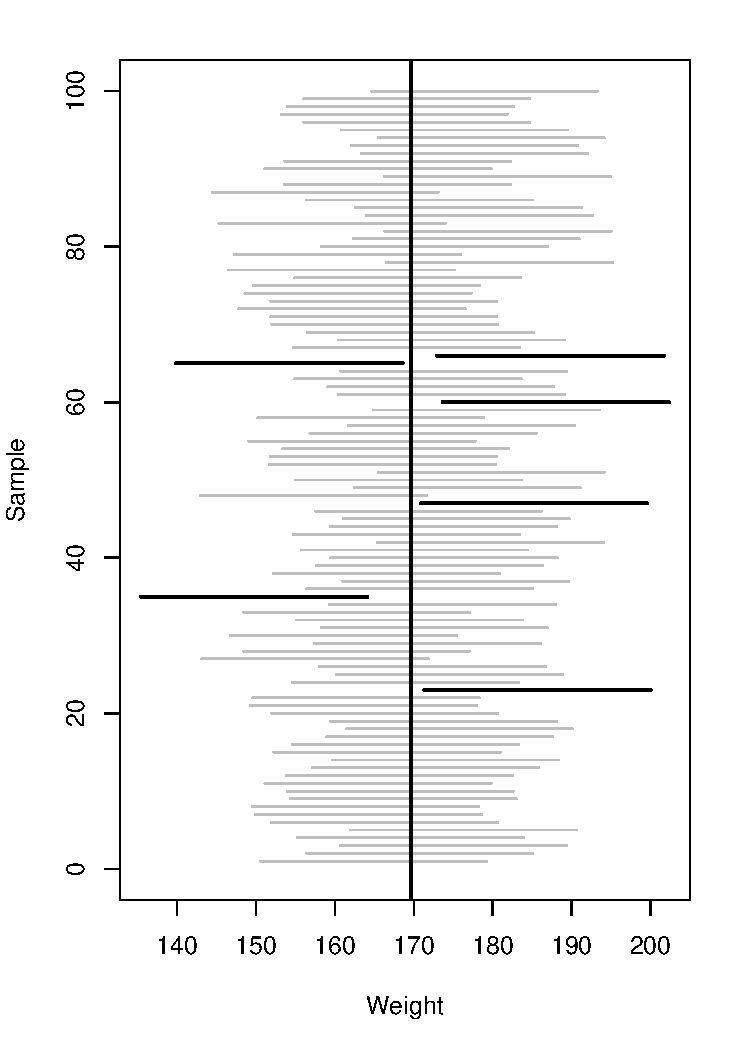
\includegraphics[width=\maxwidth]{figure/unnamed-chunk-1-1} 
\end{knitrout}

\clearpage
\textbf{Changing the confidence level}:

A $100(1-\alpha)$\% confidence interval for the population mean $\mu$ is given by
\begin{align*}
\bar{x} \pm z_{\alpha/2} \frac{\sigma}{\sqrt{n}}
\end{align*}

Here, we assume that the population size $n$ is sufficiently large so the CLT applies.  Also, since $n$ is large, when $\sigma$ is unknown, we can replace it with $s$ to obtain an approximate interval.\\

$z_{\alpha / 2}$ is the value such that $P(-z_{\alpha/2} < Z < z_{\alpha/2}) = 1-\alpha$, where $Z \sim N(0,1)$.

\begin{knitrout}
\definecolor{shadecolor}{rgb}{0.969, 0.969, 0.969}\color{fgcolor}
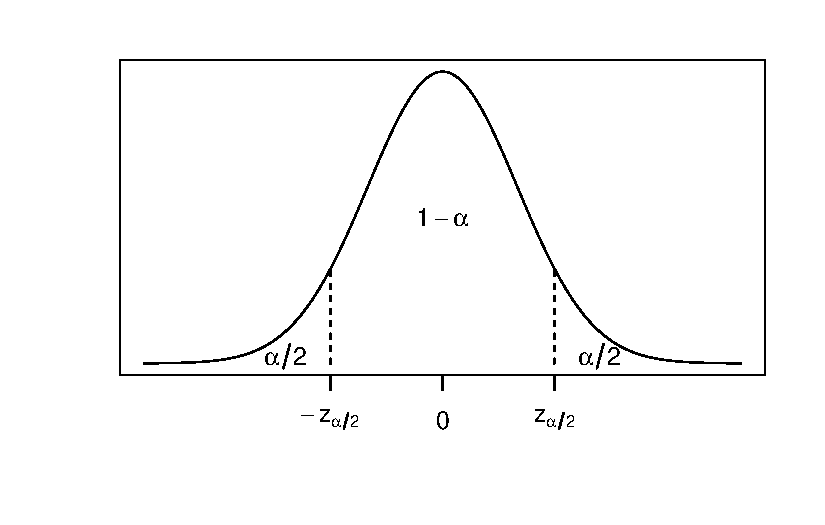
\includegraphics[width=\maxwidth]{figure/unnamed-chunk-2-1} 
\end{knitrout}

\begin{table}[ht]
\begin{tabular}{|l|l|l|}
\hline
Confidence level & Value of & $z_{\alpha/2}$\\
$1-\alpha$ & $\alpha/2$ & \\
\hline
0.9 & 0.05 & 1.645\\
0.95 & 0.025 & 1.96\\
0.98 & 0.01 & 2.326\\
0.99 & 0.005 & 2.576\\
\hline
\end{tabular}
\end{table}
The values in this table can be computed using the R command:\\
$z_{\alpha/2} = \texttt{qnorm(1-alpha/2)}$\\
\clearpage

\textbf{Ex3}: Calculate a 99\% confidence interval for the population mean number of physically active days per week for US high school students.  Recall,  the sample size $n=100$, sample mean $\bar{x} = 3.75$ days, and the sample standard deviation $s=2.6$ days.\\ 
% {\color{blue}
% For the critical value use $z_{\alpha / 2} = z_{0.005} = \texttt{qnorm(0.995)} = 2.576$\\
% $$\bar{x} \pm z_{\alpha/2} \frac{s}{\sqrt{n}} \implies
% 3.75 \pm 2.576 \cdot \frac{2.6}{\sqrt{100}}
% \implies (3.08, 4.42)$$
% }
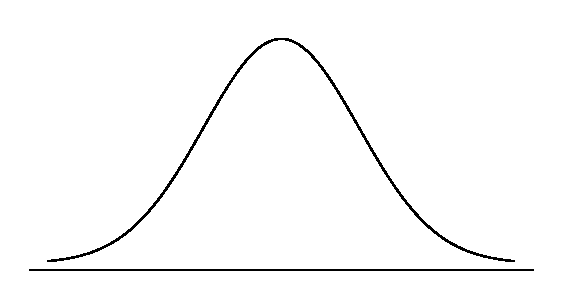
\includegraphics[scale=0.6]{norm_draw.pdf}
\vspace{2.5cm}

\textbf{Some Terminology}\\
A $100(1-\alpha)$\% confidence interval for the population mean $\mu$:
\begin{align*}
\bar{x} \pm z_{\alpha/2} \frac{\sigma}{\sqrt{n}}
\end{align*}
\begin{itemize}
\item Standard Error = SE = $\sigma/\sqrt{n}$ 
\item Margin of Error = $z_{\alpha/2} \text{SE}$ = $z_{\alpha/2} \frac{\sigma}{\sqrt{n}}$
\item Confidence Level = $1-\alpha$ (or $100(1-\alpha)$\% when expressed as a percentage)
\item $z_{\alpha/2}$ is called the critical value\\
\end{itemize}

\smallskip
\textbf{Sample Size Determination}\\
Suppose we want to estimate a confidence interval for $\mu$ with a specified margin of error.  What sample size $n$ is required so that the margin of error of the interval is $\pm$ E with confidence level~$1-\alpha$?\\

% {\color{blue}
% We can write the confidence interval as $\bar{x} \pm E$ where $E = z_{\alpha/2} \sigma / \sqrt{n}$. Solve this equation for $n$ to determine the sample size:
% \begin{align*}
% n = \left( \frac{z_{\alpha/2} \sigma}{E} \right)^2
% \end{align*}
% \textbf{Remark}: The population standard deviation $\sigma$ is usually unknown.  We can use previously collected data to calculate the sample standard deviation $s$, and then plug in $s$ as the estimate for $\sigma$ in the sample size formula.\\
% }
\clearpage

\textbf{Ex4}:  What sample size is needed to estimate the mean number of physically active days per week for US high school students using a 95\% confidence interval with a $\pm 0.25$ margin of error?\\  Use $s=2.6$ as the estimate for $\sigma$.
% \vspace{4cm}
{\color{blue}
\begin{align*}
n = \left( \frac{z_{\alpha/2} s}{E} \right)^2
= \left( \frac{1.96 \cdot 2.6}{0.25} \right)^2
= 415.5
\end{align*}
Need to sample $n = 416$ high school students.\\
}

\begin{center} 
\rule{5in}{0.4pt}
\end{center}

\textbf{Practice Problems}\\

\textbf{Practice Problem 1}:  The 2010 General Social Survey asked the question: ``For how many days during the past 30 days was your mental health, which includes stress, depression, and problems with emotions, not good?" Based on responses from 1,151 US residents, the survey reported a 95\% confidence interval of 3.40 to 4.24 days in 2010.
\begin{enumerate}[(a)]
\item Interpret this interval in context of the data.
\item Suppose the researcher thinks a 99\% confidence level would be more appropriate. Will this new interval be smaller or larger than the 95\% confidence interval?
\item If a new survey were to be done with 500 Americans, would the standard error of the estimate be larger, smaller, or about the same. Assume the standard deviation has remained constant since 2010.\\
\end{enumerate}

\textbf{Practice Problem 2}: Suppose 20 years ago, the mean cholesterol level of adult men in a certain town was 185 mg/dl with a standard deviation of 50 mg/dl.
\begin{enumerate}[(a)]
\item Suppose you obtain a random sample of size 100 and find the mean cholesterol to be\\ $\bar{x} = 210$.  Assuming that $\sigma$ has not changed, find a 90\% confidence interval for the mean cholesterol level of the population (of adult men in this town).
\item Suppose you decide to conduct a new study to determine the mean cholesterol level of adult men in this town.  Assuming that the standard deviation has not changed, how many people should you include in your sample if you want the margin of error to be $\pm 10$ mg/dl, using 95\% confidence.
\item If you want to be 99\% confident, then how large should your sample size be?\\
\end{enumerate}

\textbf{Practice Problem 3}: In any given situation, if the level of confidence and the standard deviation are kept constant, how much would you need to increase the sample size to decrease the width of the interval to half its original size?\\

\newpage

\textbf{Solutions to Practice Problems}\\

\textbf{Practice Problem 1}
\begin{enumerate}[(a)]
\item We are 95\% confident that the population mean $\mu$ for the number of days per month US residents report being in poor mental health is between 3.4 and 4.24.
\item A 99\% confidence interval would be larger.
\item The standard error $SE=\sigma / \sqrt{n}$ would be larger since when $n$ decreases the SE will increase, assuming $\sigma$ is fixed.\\
\end{enumerate}

\textbf{Practice Problem 2}
\begin{enumerate}[(a)]
\item
Since $n$ is large ($\geq 30$), and the sample is random, the confidence interval is valid by the CLT.  Thus a 90\% confidence interval for $\mu$ is given by\\
\begin{align*}
\bar{x} \pm z_{\alpha/2} \frac{\sigma}{\sqrt{n}} \implies 210 \pm 1.645 \frac{50}{\sqrt{100}} \implies (201.775, 218.225)
\end{align*}
\item
\begin{align*}
n = \left(\frac{z_{\alpha/2} \sigma}{E} \right)^2 = \left( \frac{1.96\cdot 50}{10} \right)^2 = 96.04
\end{align*}
A sample size of 96 is needed.\\
\item
\begin{align*}
n = \left(\frac{z_{\alpha/2} \sigma}{E} \right)^2 = \left( \frac{2.576\cdot 50}{10} \right)^2 = 165.9
\end{align*}
A sample size of 166 is needed.\\
\end{enumerate}

\textbf{Practice Problem 3}\\
You would need to increase the sample size $n$ by a factor of 4.  The margin of error $E = z_{\alpha/2} \sigma / \sqrt{n}$.  Substituting $4n$ into the margin of error formula gives
\begin{align*}
z_{\alpha/2} \frac{\sigma}{\sqrt{4n}} = z_{\alpha/2} \frac{\sigma}{2\sqrt{n}} = \frac{E}{2}\\
\end{align*}

\clearpage

\textbf{Code Appendix}

Here is the code I wrote to visualize confidence intervals (for mean weight) constructed by repeatedly taking samples from the population.  You are not expected to know how to make a plot like this; but I decided to include the code in case you are interested.

\begin{knitrout}
\definecolor{shadecolor}{rgb}{0.969, 0.969, 0.969}\color{fgcolor}\begin{kframe}
\begin{alltt}
\hlstd{cdc} \hlkwb{<-} \hlkwd{readRDS}\hlstd{(}\hlkwd{url}\hlstd{(}\hlstr{"https://ericwfox.github.io/data/cdc.rds"}\hlstd{))}

\hlkwd{set.seed}\hlstd{(}\hlnum{200}\hlstd{)}
\hlstd{mu} \hlkwb{<-} \hlkwd{mean}\hlstd{(cdc}\hlopt{$}\hlstd{weight)}
\hlstd{sigma} \hlkwb{<-} \hlkwd{sd}\hlstd{(cdc}\hlopt{$}\hlstd{weight)}
\hlstd{ci_lower} \hlkwb{<-} \hlkwd{rep}\hlstd{(}\hlnum{0}\hlstd{,} \hlnum{100}\hlstd{)}
\hlstd{ci_upper} \hlkwb{<-} \hlkwd{rep}\hlstd{(}\hlnum{0}\hlstd{,} \hlnum{100}\hlstd{)}
\hlstd{contains} \hlkwb{<-} \hlkwd{rep}\hlstd{(}\hlnum{0}\hlstd{,} \hlnum{100}\hlstd{)}
\hlkwa{for}\hlstd{(i} \hlkwa{in} \hlnum{1}\hlopt{:}\hlnum{100}\hlstd{) \{}
  \hlstd{samp} \hlkwb{<-} \hlkwd{sample}\hlstd{(cdc}\hlopt{$}\hlstd{weight,} \hlnum{30}\hlstd{)}
  \hlstd{ci_lower[i]} \hlkwb{<-} \hlkwd{mean}\hlstd{(samp)} \hlopt{-} \hlnum{1.96} \hlopt{*} \hlstd{sigma} \hlopt{/} \hlkwd{sqrt}\hlstd{(}\hlnum{30}\hlstd{)}
  \hlstd{ci_upper[i]} \hlkwb{<-} \hlkwd{mean}\hlstd{(samp)} \hlopt{+} \hlnum{1.96} \hlopt{*} \hlstd{sigma} \hlopt{/} \hlkwd{sqrt}\hlstd{(}\hlnum{30}\hlstd{)}
  \hlkwa{if}\hlstd{(mu} \hlopt{>=} \hlstd{ci_lower[i]} \hlopt{&} \hlstd{mu} \hlopt{<=} \hlstd{ci_upper[i]) \{}
    \hlstd{contains[i]} \hlkwb{<-} \hlnum{1}
  \hlstd{\}}
\hlstd{\}}

\hlkwd{par}\hlstd{(}\hlkwc{mar}\hlstd{=}\hlkwd{c}\hlstd{(}\hlnum{5}\hlstd{,} \hlnum{4}\hlstd{,} \hlnum{2}\hlstd{,} \hlnum{2}\hlstd{))} \hlcom{# format margins}
\hlstd{xmin} \hlkwb{<-} \hlkwd{min}\hlstd{(ci_lower)}
\hlstd{xmax} \hlkwb{<-} \hlkwd{max}\hlstd{(ci_upper)}
\hlkwd{plot}\hlstd{(}\hlkwd{c}\hlstd{(xmin, xmax),} \hlkwd{c}\hlstd{(}\hlnum{0}\hlstd{,} \hlnum{100}\hlstd{),} \hlkwc{type}\hlstd{=}\hlstr{"n"}\hlstd{,} \hlkwc{xlab} \hlstd{=} \hlstr{"Weight"}\hlstd{,} \hlkwc{ylab} \hlstd{=} \hlstr{"Sample"}\hlstd{)}
\hlkwa{for}\hlstd{(i} \hlkwa{in} \hlnum{1}\hlopt{:}\hlnum{100}\hlstd{) \{}
  \hlkwd{lines}\hlstd{(}\hlkwd{c}\hlstd{(ci_lower[i], ci_upper[i]),} \hlkwd{c}\hlstd{(i, i),} \hlkwc{col}\hlstd{=}\hlstr{"grey"}\hlstd{,} \hlkwc{lwd}\hlstd{=}\hlnum{1.25}\hlstd{)}
  \hlkwa{if}\hlstd{(contains[i]} \hlopt{==} \hlnum{0}\hlstd{) \{}
    \hlkwd{lines}\hlstd{(}\hlkwd{c}\hlstd{(ci_lower[i], ci_upper[i]),} \hlkwd{c}\hlstd{(i, i),} \hlkwc{col}\hlstd{=}\hlstr{"black"}\hlstd{,} \hlkwc{lwd}\hlstd{=}\hlnum{2}\hlstd{)}
  \hlstd{\}}
\hlstd{\}}
\hlkwd{abline}\hlstd{(}\hlkwc{v}\hlstd{=mu,} \hlkwc{col}\hlstd{=}\hlstr{"black"}\hlstd{,} \hlkwc{lwd}\hlstd{=}\hlnum{2}\hlstd{)}
\end{alltt}
\end{kframe}
\end{knitrout}






\end{document}
